\chapter{Results}
\label{chap:Results}
%importanza loop (cambio stato), confronto a cambio di loop
%discutere i loops e i vari risultati
%noi non prendiamo codici di errorere, ma solo coverage
%punti di forza e debolezza di fallaway
%aflnet e chatafl quasi lineare
%fallaway ha un andamento a scalini, piu' casuale
\begin{itemize}
    \item Fallaway:
    \begin{lstlisting}

    complete_coverage: 6% (883/15168)
    total_executions: 79987763
    \end{lstlisting}
    
    \item AFLNet:
    \begin{lstlisting}
    
    complete_coverage: 5% (830/15168)
    total_executions: 209776
    \end{lstlisting}
    
    \item ChatAFL:
    \begin{lstlisting}
    
    complete_coverage: 6% (850/15168)
    total_executions: 241242
    \end{lstlisting}
\end{itemize}
After 24h of fuzzing, we can look at the results and analyze them.
\\\textbf{Fallaway} has the highest coverage of 6\% with 883 edge cases covered.
\\It has the highest number of total executions with 79,987,763, which is 381 times more than \textbf{AFLNet} and 332 times more than \textbf{ChatAFL}.
\\\textbf{AFLNet} has the lowest coverage of 5\% with 830 edge cases covered.
\\It has the lowest number of total executions with 209,776.
\\\textbf{ChatAFL} has a coverage of 6\% with 850 edge cases covered.
\\It has a total of 241,242 executions.
\\The coverage of the three fuzzers over 24h is shown in Figure \ref{fig:coverage_1day}.

\begin{figure}[H]
    \centering
    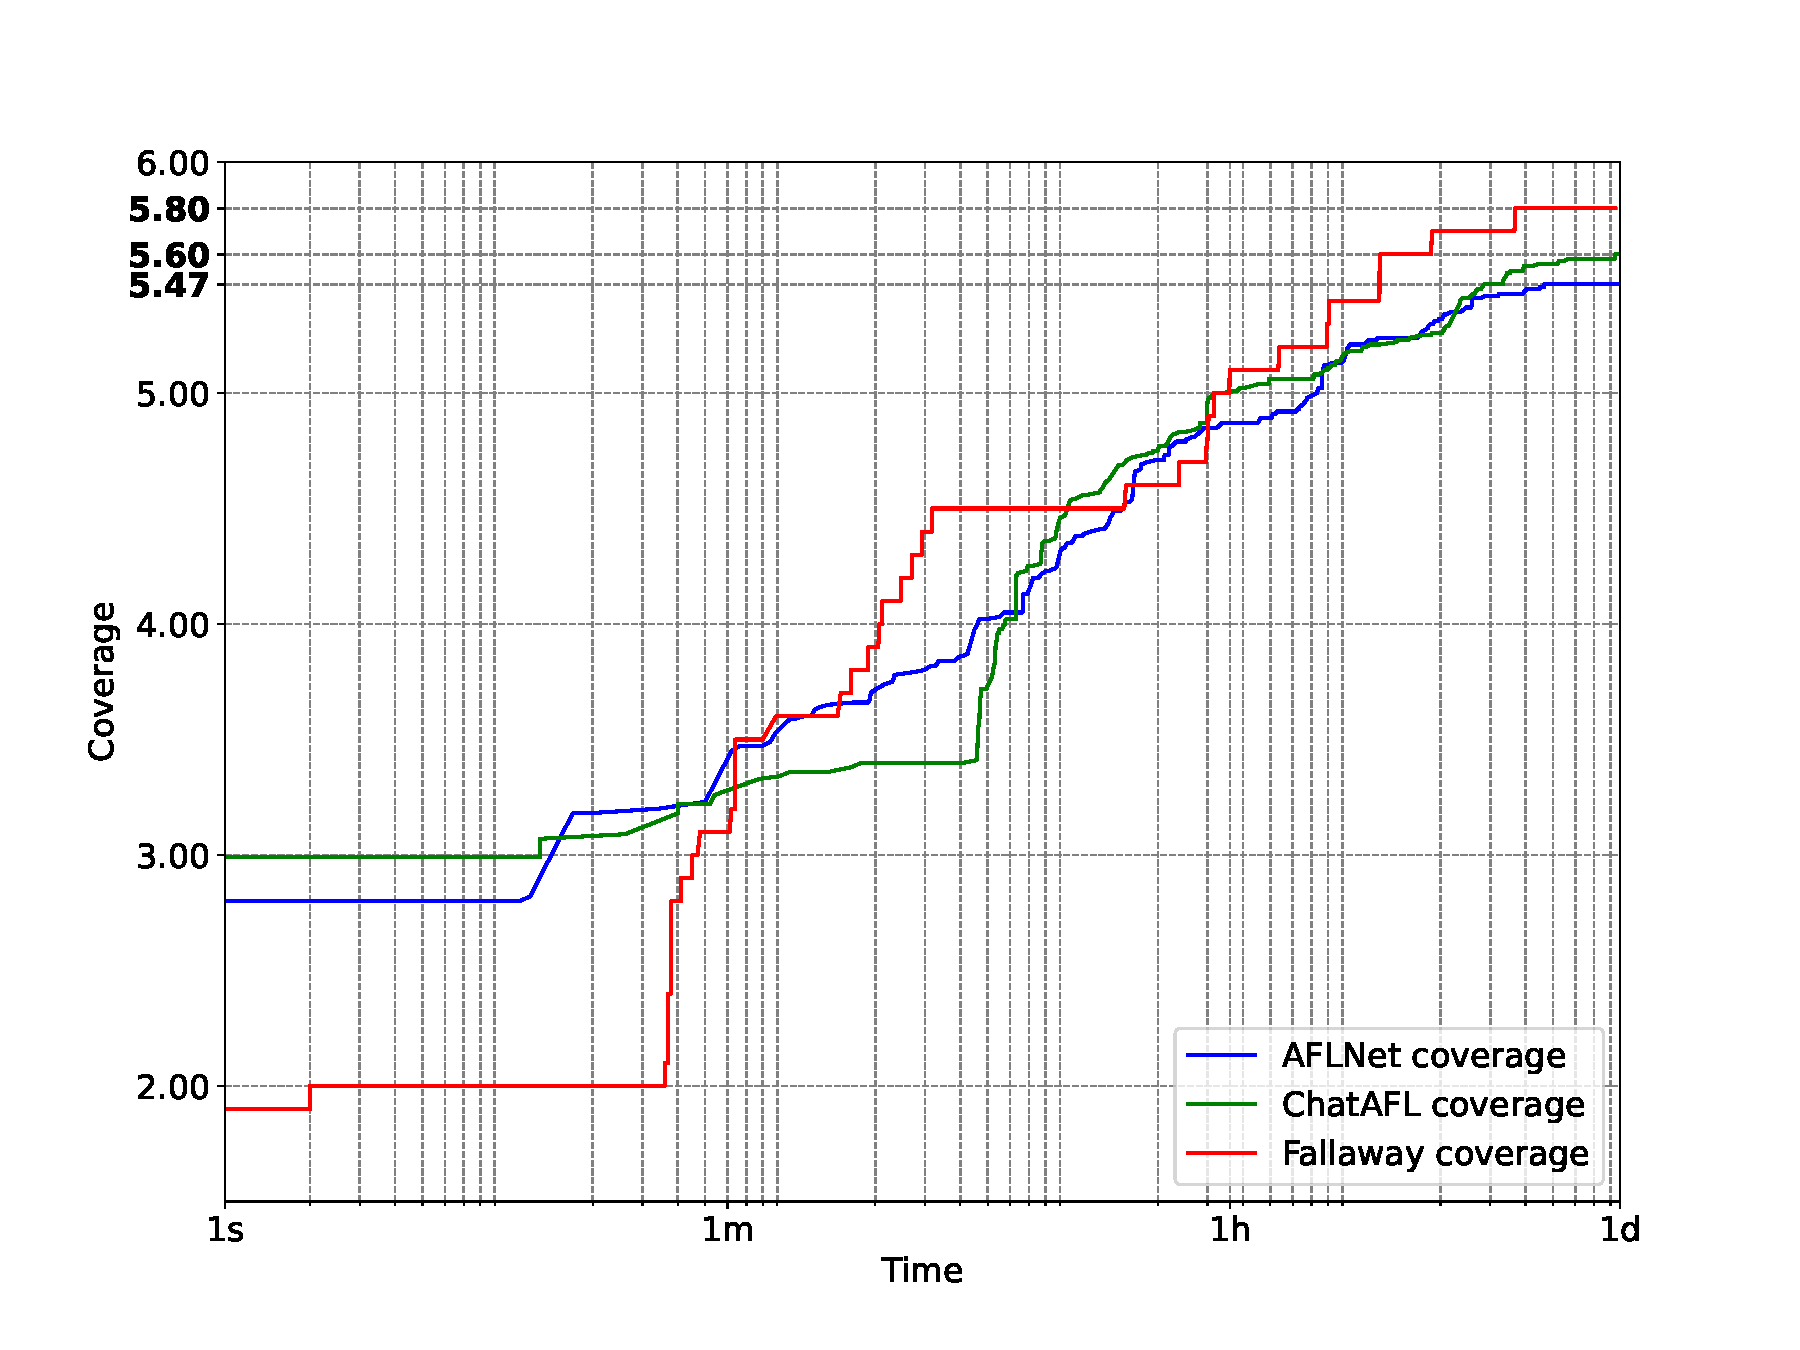
\includegraphics[width=1\textwidth]{Images/coverage_over_time_lighttpd-1day.pdf}
    \caption{Coverage of the three fuzzers in 24h}
    \label{fig:coverage_1day}
\end{figure}
\phantom{}\\
In another experiment, we ran the fuzzers for 10 hours, modifying the configuration of Fallaway to be in a loop of 250.
\\The coverage of the three fuzzers over 10h is shown in Figure \ref{fig:coverage_10hours}.

\begin{figure}[H]
    \centering
    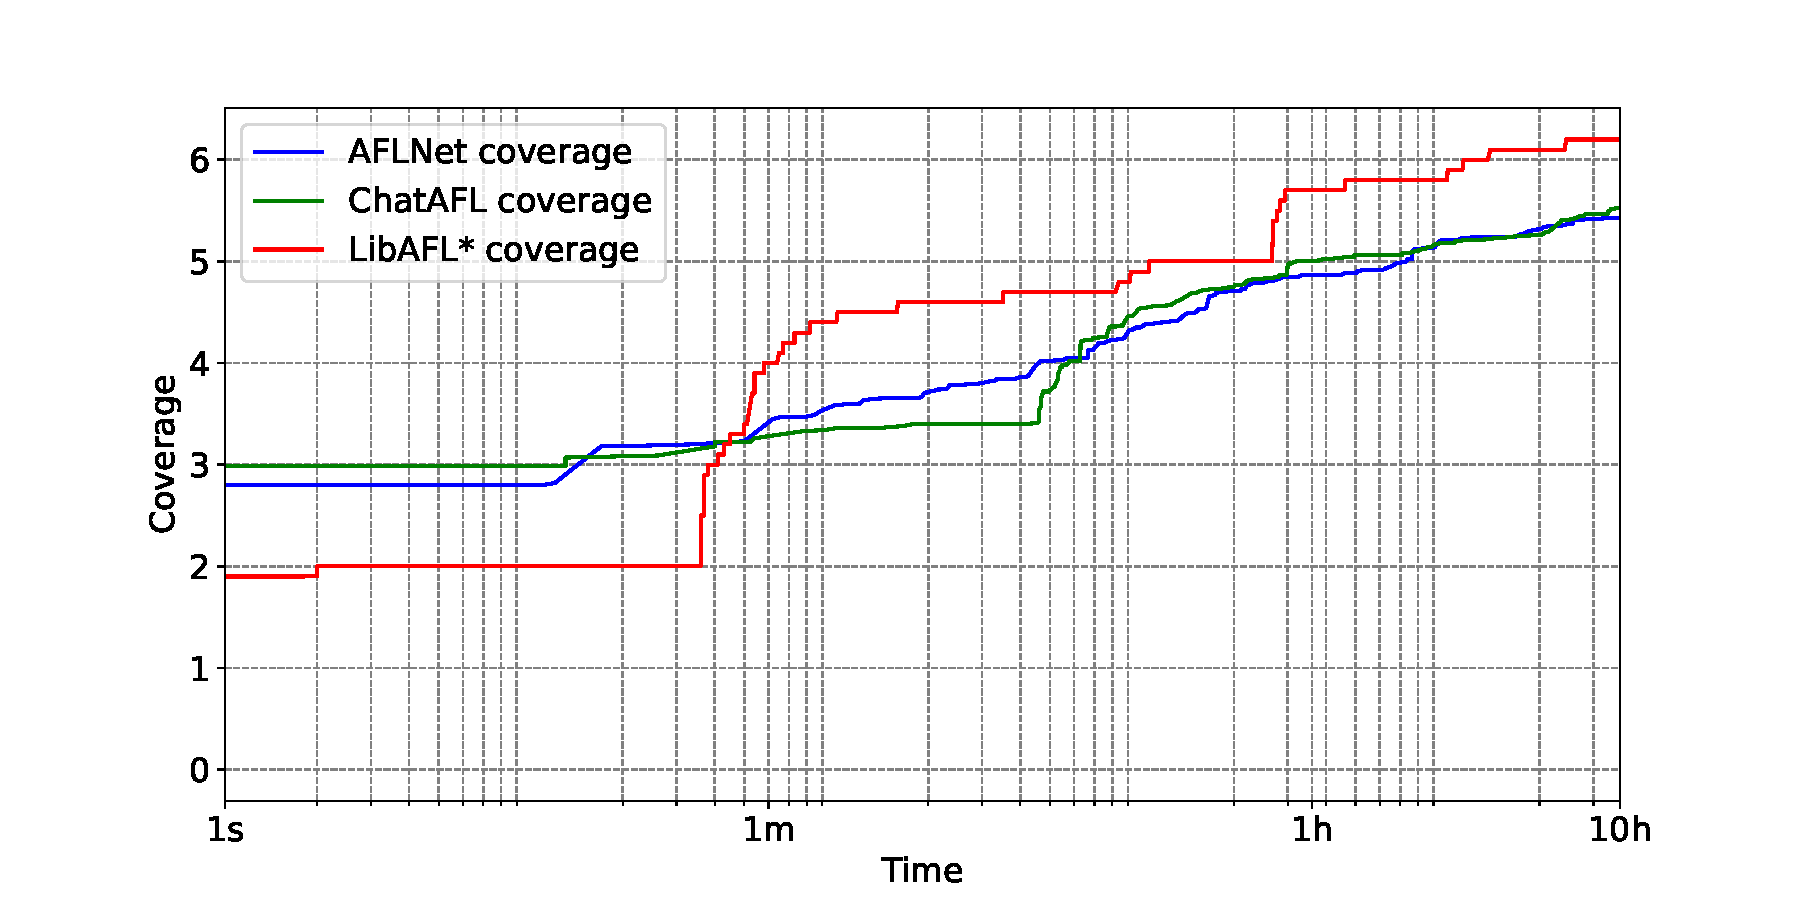
\includegraphics[width=1\textwidth]{Images/coverage_over_time_lighttpd-10h.pdf}
    \caption{Coverage of the three fuzzers in 10 hours}
    \label{fig:coverage_10hours}
\end{figure}
\phantom{}\\
In this configuration, Fallaway has reached a complete\_coverage of 6\% (942/15168).
\\This is 59 more edge cases than the previous configuration, which is a 6.7\% increase.
\\This could be due to the fact that the fuzzer is running in a loop of 250, which allows it to run more test cases in a shorter amount of time.
\\This is not always a good thing, it depends on the SUT, corpus, configurations and more because in general: higher loop values can lead to more coverage, but also to more redundant test cases and to stuck on states that makes low progress; lower loop values can lead to less coverage, but also to less redundant test cases and to faster progress.